In this section we perform various signal injection tests. We only consider the double ratio constructed as in section~\ref{ssec:all_errors_included} (i.e. with all sources of uncertainties taken into account). We consider in turn the injection of a fairly large coefficient ($d_u^{YZ} = 1.35 \times 10^{-4}$) and injected it both with a sidereal and solar phase. The former corresponds to a possible signal while the latter simulates a potential day/night effect. The purposes of these studies are:
\begin{enumerate}
    \item Test to what extent we are able to recover the signal using our 100 bins fitting procedure.
    \item Test to what extent one single scrambling of the time stamps erases the signal. This is essential for proving the feasibility of a partial unblinding of the data (i.e. using the observed $Z$ counts but scrambling the time stamps).
    \item Test the extent of the solar/sidereal phase signal cross contamination. How large of a sidereal coefficient is observed if a solar phase signal is injected (and vice versa). 
    \item Test the size of the fitted coefficient as a function of the testing phase. 
\end{enumerate}
%

\subsection{Sidereal phase signal injection: recovery test}
\label{ssec:SiderealInjectionRecovery}
%
The construction of a simulated set of $Z$ counts with an injected sideral signal is achieved by simply replacing the SM fiducial cross section in Eqs.~(\ref{eq:NZfull}) and (\ref{eq:NZcorrfull}):
%
\begin{align}
    \sigma_\text{fid} = A^\text{SM} \sigma_\text{SM}^\text{NNLO} 
    \longrightarrow
    \sigma_\text{fid} \left[ 1 + d_u^{YZ} \big[ a \cos (\omega_\oplus T_\oplus) + b \sin (\omega_\oplus T_\oplus) \big] \right]
\end{align}
%
where the numerical values for $a$ and $b$ are taken from Eq.~(\ref{eq:duYZnum}). For a solar signal we use the same formula but replace the sidereal frequency $\omega_\oplus = 2\pi/T_\text{sidereal}$ with $\omega_\odot = 2\pi/T_\text{solar} = 2\pi/(24\; \text{hr})$. The $R_D$ distribution and the fit results for a sidereal, solar and 1 hr testing phase are presented in figures~\ref{fig:RD_sidereal_signal}, \ref{fig:RD_sidereal_signal_fits_sidsol} and \ref{fig:RD_sidereal_signal_fits_1h}. 

Several comments are in order:
\begin{itemize}
\item Using the sidereal testing phase, we extract $\left[d_u^{YZ}\right]_\text{fit} = (1.25 \pm 0.05)\times 10^{-4}$ which is quite compatible with the injected signal  $\left[d_u^{YZ}\right]_\text{injected} = 1.35 \times 10^{-4}$.
\item Using the sidereal testing phase, we find large reconstructed signals for all $YZ$ coefficients (and not only for $d_u^{YZ}$) because the time structure induced by these coefficients is identical (up to an overall rescaling factor). 
\item Using the sidereal testing phases, no coefficient other than the $YZ$ ones deviates from zero. Because of linearity, this demonstrates that, if multiple coefficients are present (e.g. a $YZ$ and an $XY$), they can all be identified (of course, we cannot distinguish between $c_d$, $c_u$ and $d_u$).
\item As can be seen in the right side of figure~\ref{fig:RD_sidereal_signal_fits_sidsol}, a large sidereal signal will induce (smaller) but still sizable solar day effects. 
\end{itemize}

\begin{figure}[H]
\centering
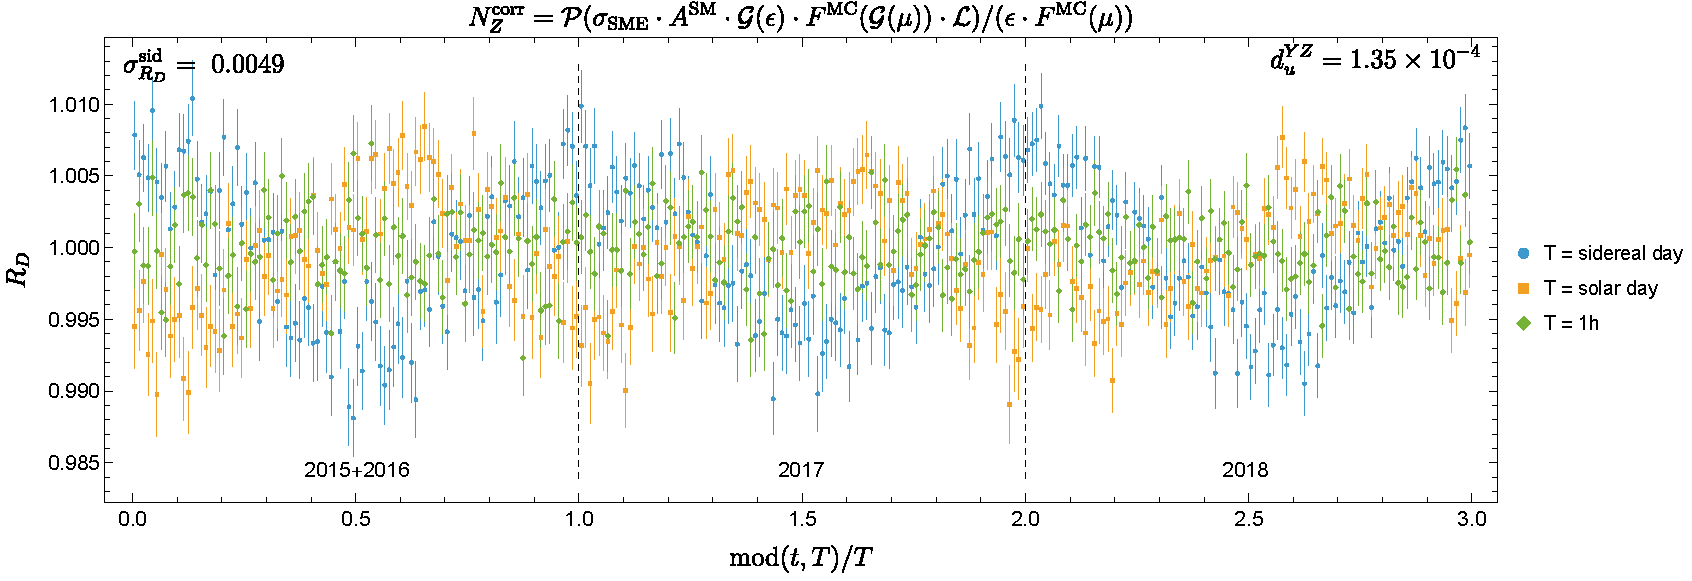
\includegraphics[width=\textwidth]{figs/Mathematica-oldchi2/xs(sigmaFIDSME eps FMC)_phase}
\caption{$R_D$ distribution with a sidereal signal injection ($d_u^{YZ} = 1.35 \times 10^{-4}$). In the upper right corner we show the standard deviation of the sidereal day distribution.}
\label{fig:RD_sidereal_signal}
\end{figure}

\begin{figure}[H]
\centering
\begin{minipage}[H]{\textwidth}
    \vspace{0pt}
    \centering
   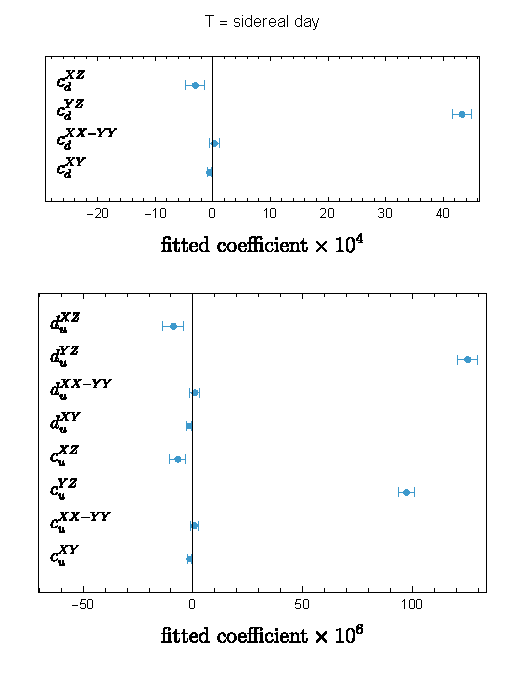
\includegraphics[width=0.49\textwidth]{figs/Mathematica-oldchi2/xs(sigmaFIDSME eps FMC)_fit_sday}
   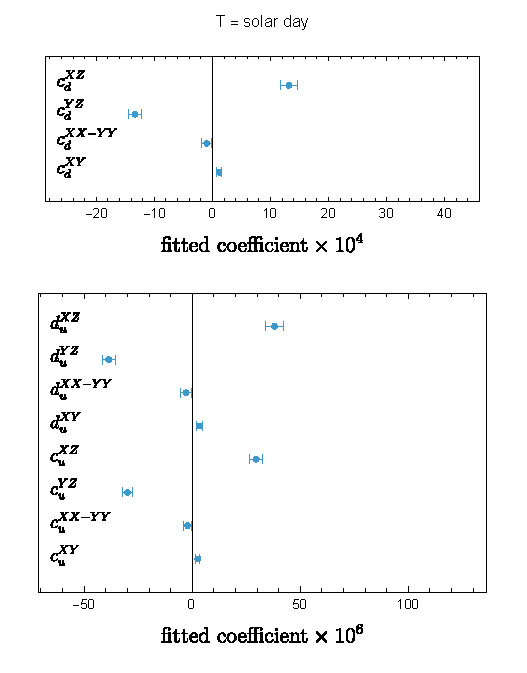
\includegraphics[width=0.49\textwidth]{figs/Mathematica-oldchi2/xs(sigmaFIDSME eps FMC)_fit_day}
\end{minipage}
\begin{minipage}[H]{\textwidth}
    \vspace{1.6cm}
    \centering
    \begin{tabular}{|l|c|}
        \hline
        $d_u^{XZ}$ & $(-8.9 \pm 4.8)\times 10^{-6}$ \\
        $d_u^{YZ}$ & $(1.252 \pm 0.046)\times 10^{-4}$ \\
        $d_u^{XX-YY}$ & $(0.9 \pm 2.4)\times 10^{-6}$ \\
        $d_u^{XY}$ & $(-1.8 \pm 1.1)\times 10^{-6}$ \\
        $c_u^{XZ}$ & $(-6.9 \pm 3.7)\times 10^{-6}$ \\
        $c_u^{YZ}$ & $(9.73 \pm 0.36)\times 10^{-5}$ \\
        $c_u^{XX-YY}$ & $(0.7 \pm 1.8)\times 10^{-6}$ \\
        $c_u^{XY}$ & $(-1.40 \pm 0.89)\times 10^{-6}$ \\
        $c_d^{XZ}$ & $(-3.1 \pm 1.7)\times 10^{-4}$ \\
        $c_d^{YZ}$ & $(4.33 \pm 0.16)\times 10^{-3}$ \\
        $c_d^{XX-YY}$ & $(3.0 \pm 8.1)\times 10^{-5}$ \\
        $c_d^{XY}$ & $(-6.2 \pm 4.0)\times 10^{-5}$ \\
                \hline
        \end{tabular}
        \;\;\;\;\;\;\;\;\;\;\;\;\;\;\;\;\;\;
    \begin{tabular}{|l|c|}
        \hline
        $d_u^{XZ}$ & $(3.81 \pm 0.41)\times 10^{-5}$ \\
        $d_u^{YZ}$ & $(-3.86 \pm 0.32)\times 10^{-5}$ \\
        $d_u^{XX-YY}$ & $(-2.8 \pm 2.4)\times 10^{-6}$ \\
        $d_u^{XY}$ & $(3.4 \pm 1.2)\times 10^{-6}$ \\
        $c_u^{XZ}$ & $(2.96 \pm 0.32)\times 10^{-5}$ \\
        $c_u^{YZ}$ & $(-3.00 \pm 0.25)\times 10^{-5}$ \\
        $c_u^{XX-YY}$ & $(-2.2 \pm 1.9)\times 10^{-6}$ \\
        $c_u^{XY}$ & $(2.61 \pm 0.90)\times 10^{-6}$ \\
        $c_d^{XZ}$ & $(1.32 \pm 0.14)\times 10^{-3}$ \\
        $c_d^{YZ}$ & $(-1.33 \pm 0.11)\times 10^{-3}$ \\
        $c_d^{XX-YY}$ & $(-9.8 \pm 8.4)\times 10^{-5}$ \\
        $c_d^{XY}$ & $(1.16 \pm 0.40)\times 10^{-4}$ \\
                        \hline
        \end{tabular}
\end{minipage}
\caption{Sidereal signal injection test ($d_u^{YZ} = 1.35 \times 10^{-4}$): fit results for sidereal (left) and solar (right) testing phases.}
\label{fig:RD_sidereal_signal_fits_sidsol}
\end{figure}

\begin{figure}[H]
\centering
\begin{minipage}[H]{0.49\textwidth}
    \vspace{1.6cm}
    \centering
    \begin{tabular}{|l|c|}
        \hline
        $d_u^{XZ}$ & $(-5.0 \pm 4.8)\times 10^{-6}$ \\
        $d_u^{YZ}$ & $(2.9 \pm 4.8)\times 10^{-6}$ \\
        $d_u^{XX-YY}$ & $(1.3 \pm 2.5)\times 10^{-6}$ \\
        $d_u^{XY}$ & $(6. \pm 12.)\times 10^{-7}$ \\
        $c_u^{XZ}$ & $(-3.9 \pm 3.7)\times 10^{-6}$ \\
        $c_u^{YZ}$ & $(2.3 \pm 3.7)\times 10^{-6}$ \\
        $c_u^{XX-YY}$ & $(1.0 \pm 1.9)\times 10^{-6}$ \\
        $c_u^{XY}$ & $(4.9 \pm 9.5)\times 10^{-7}$ \\
        $c_d^{XZ}$ & $(-1.7 \pm 1.7)\times 10^{-4}$ \\
        $c_d^{YZ}$ & $(1.0 \pm 1.7)\times 10^{-4}$ \\
        $c_d^{XX-YY}$ & $(4.5 \pm 8.5)\times 10^{-5}$ \\
        $c_d^{XY}$ & $(2.2 \pm 4.2)\times 10^{-5}$ \\
        \hline
        \end{tabular}
\end{minipage}
\begin{minipage}[H]{0.49\textwidth}
    \vspace{0pt}
    \centering
   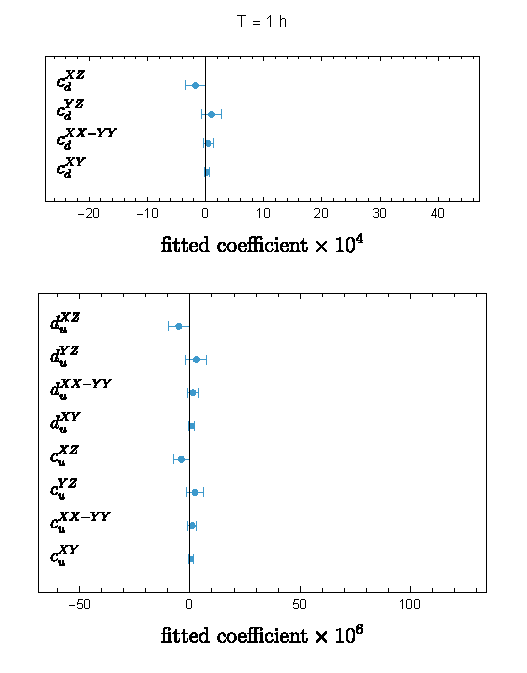
\includegraphics[width=\textwidth]{figs/Mathematica-oldchi2/xs(sigmaFIDSME eps FMC)_fit_1h}
\end{minipage}
\caption{Sidereal signal injection test ($d_u^{YZ} = 1.35 \times 10^{-4}$): fit results for 1 hr testing phase.}
\label{fig:RD_sidereal_signal_fits_1h}
\end{figure}

\subsection{Sidereal phase signal injection: scrambling}
\label{ssec:SiderealInjectionScrambling}
%
In figures~\ref{fig:RD_sidereal_signal_scrambled} and \ref{fig:RD_sidereal_signal_scrambled_fits_sidsol}, we demonstrate that a random scrambling of all time stamps is sufficient to completely erase the presence of a strong sidereal signal. Note that, after scrambling, the standard deviation over the 100 bins in $R_D$ drops from 0.0049 to 0.0026 (which is typical of a SM simulation without signal injection). 

\begin{figure}[H]
\centering
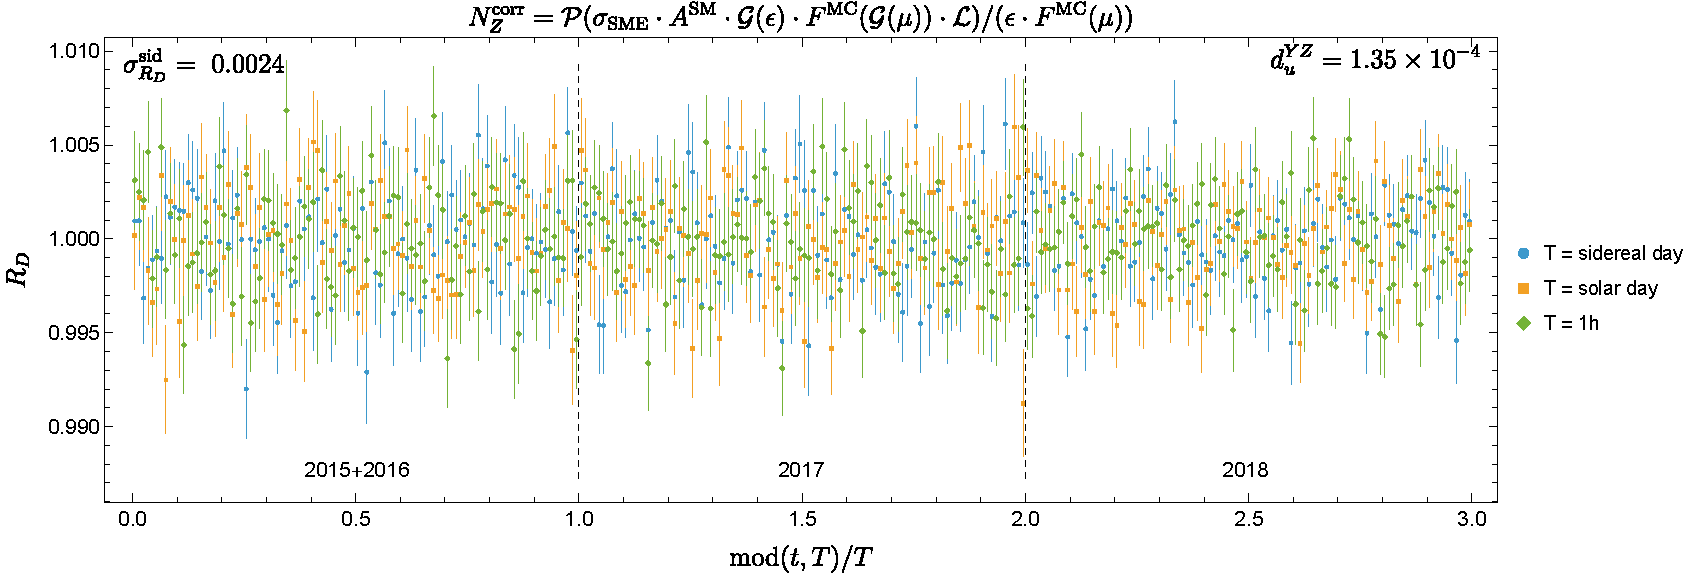
\includegraphics[width=\textwidth]{figs/Mathematica-oldchi2/xs(sigmaFIDSME eps FMC)_randomized_phase}
\caption{$R_D$ distribution with a sidereal signal injection ($d_u^{YZ} = 1.35 \times 10^{-4}$) after one scrambling. In the upper right corner we show the standard deviation of the sidereal day distribution.}
\label{fig:RD_sidereal_signal_scrambled}
\end{figure}


\begin{figure}[H]
\centering
\begin{minipage}[H]{\textwidth}
    \vspace{0pt}
    \centering
   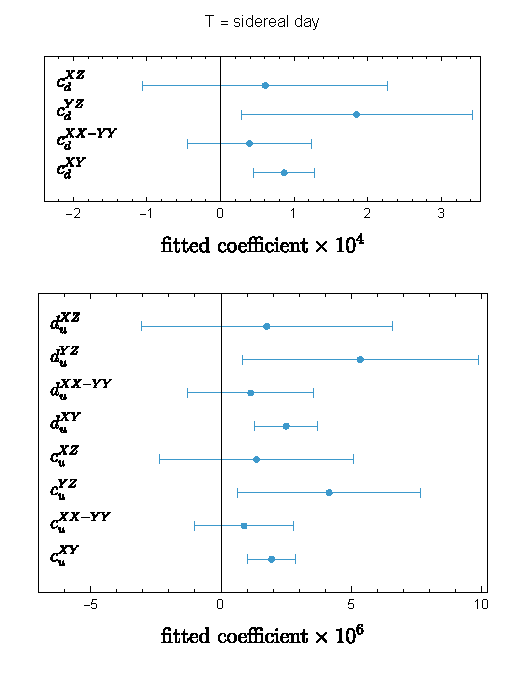
\includegraphics[width=0.49\textwidth]{figs/Mathematica-oldchi2/xs(sigmaFIDSME eps FMC)_randomized_fit_sday}
   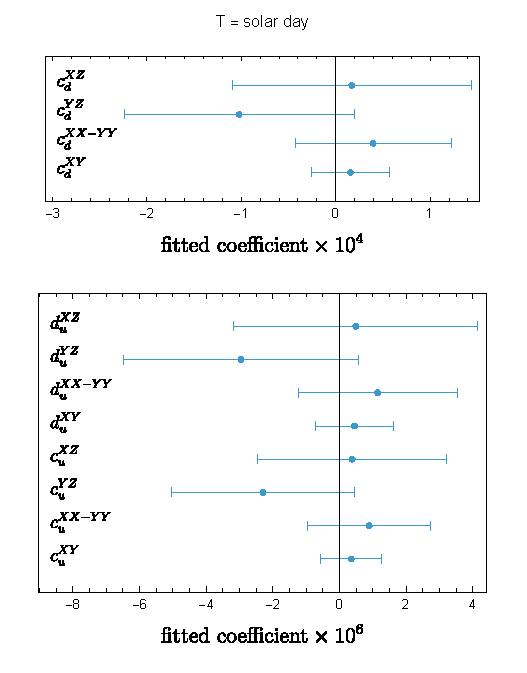
\includegraphics[width=0.49\textwidth]{figs/Mathematica-oldchi2/xs(sigmaFIDSME eps FMC)_randomized_fit_day}
\end{minipage}
\begin{minipage}[H]{\textwidth}
    \vspace{1.6cm}
    \centering
    \begin{tabular}{|l|c|}
        \hline
        $d_u^{XZ}$ & $(-8.9 \pm 4.8)\times 10^{-6}$ \\
        $d_u^{YZ}$ & $(1.252 \pm 0.046)\times 10^{-4}$ \\
        $d_u^{XX-YY}$ & $(0.9 \pm 2.4)\times 10^{-6}$ \\
        $d_u^{XY}$ & $(-1.8 \pm 1.1)\times 10^{-6}$ \\
        $c_u^{XZ}$ & $(-6.9 \pm 3.7)\times 10^{-6}$ \\
        $c_u^{YZ}$ & $(9.73 \pm 0.36)\times 10^{-5}$ \\
        $c_u^{XX-YY}$ & $(0.7 \pm 1.8)\times 10^{-6}$ \\
        $c_u^{XY}$ & $(-1.40 \pm 0.89)\times 10^{-6}$ \\
        $c_d^{XZ}$ & $(-3.1 \pm 1.7)\times 10^{-4}$ \\
        $c_d^{YZ}$ & $(4.33 \pm 0.16)\times 10^{-3}$ \\
        $c_d^{XX-YY}$ & $(3.0 \pm 8.1)\times 10^{-5}$ \\
        $c_d^{XY}$ & $(-6.2 \pm 4.0)\times 10^{-5}$ \\
                \hline
        \end{tabular}
        \;\;\;\;\;\;\;\;\;\;\;\;\;\;\;\;\;\;
    \begin{tabular}{|l|c|}
        \hline
        $d_u^{XZ}$ & $(3.81 \pm 0.41)\times 10^{-5}$ \\
        $d_u^{YZ}$ & $(-3.86 \pm 0.32)\times 10^{-5}$ \\
        $d_u^{XX-YY}$ & $(-2.8 \pm 2.4)\times 10^{-6}$ \\
        $d_u^{XY}$ & $(3.4 \pm 1.2)\times 10^{-6}$ \\
        $c_u^{XZ}$ & $(2.96 \pm 0.32)\times 10^{-5}$ \\
        $c_u^{YZ}$ & $(-3.00 \pm 0.25)\times 10^{-5}$ \\
        $c_u^{XX-YY}$ & $(-2.2 \pm 1.9)\times 10^{-6}$ \\
        $c_u^{XY}$ & $(2.61 \pm 0.90)\times 10^{-6}$ \\
        $c_d^{XZ}$ & $(1.32 \pm 0.14)\times 10^{-3}$ \\
        $c_d^{YZ}$ & $(-1.33 \pm 0.11)\times 10^{-3}$ \\
        $c_d^{XX-YY}$ & $(-9.8 \pm 8.4)\times 10^{-5}$ \\
        $c_d^{XY}$ & $(1.16 \pm 0.40)\times 10^{-4}$ \\
                        \hline
        \end{tabular}
\end{minipage}
\caption{Sidereal signal injection test ($d_u^{YZ} = 1.35 \times 10^{-4}$) after one scrambling of all time stamps: fit results for sidereal (left) and solar (right) testing phases.}
\label{fig:RD_sidereal_signal_scrambled_fits_sidsol}
\end{figure}



\subsection{Sidereal phase signal injection: scan over the testing phase}
\label{ssec:SiderealInjectionScan}
%
In this section we study, as a function of the testing phase, the extraction of the coefficient $d_u^{YZ}$ from a sample in which a $d_u^{YZ} = 1.35 \times 10^{-4}$ sidereal signal has been injected. The results of this test is presented in figure~\ref{fig:RD_sidereal_signal_scan} (the four lower panels focus on the restricted [23 hr, 25 hr] range). Around the sidereal and solar phases we scan the testing phase with a granularity of 1 min (going below this is problematic because the average LB duration is about 1 min). 

This analysis suggests a possible strategy to decide whether a positive observation is a genuine sidereal signal or a day/night effect: just check whether the largest extracted coefficient is the output of a sidereal or solar testing phase. 

\begin{figure}[H]
\centering
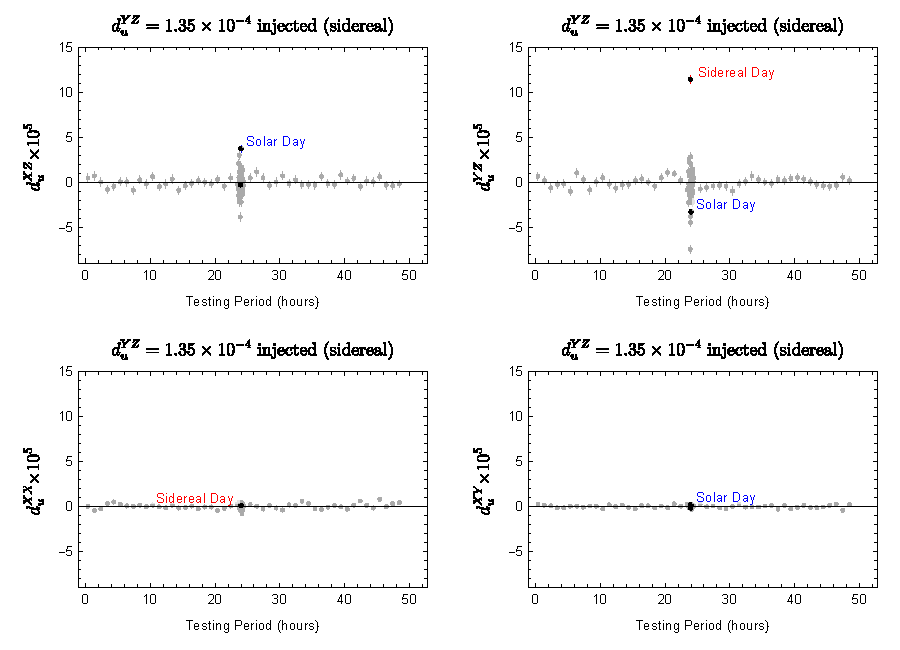
\includegraphics[width=0.8\textwidth]{figs/Mathematica-oldchi2/fit_duYZinjected_scan-wide}
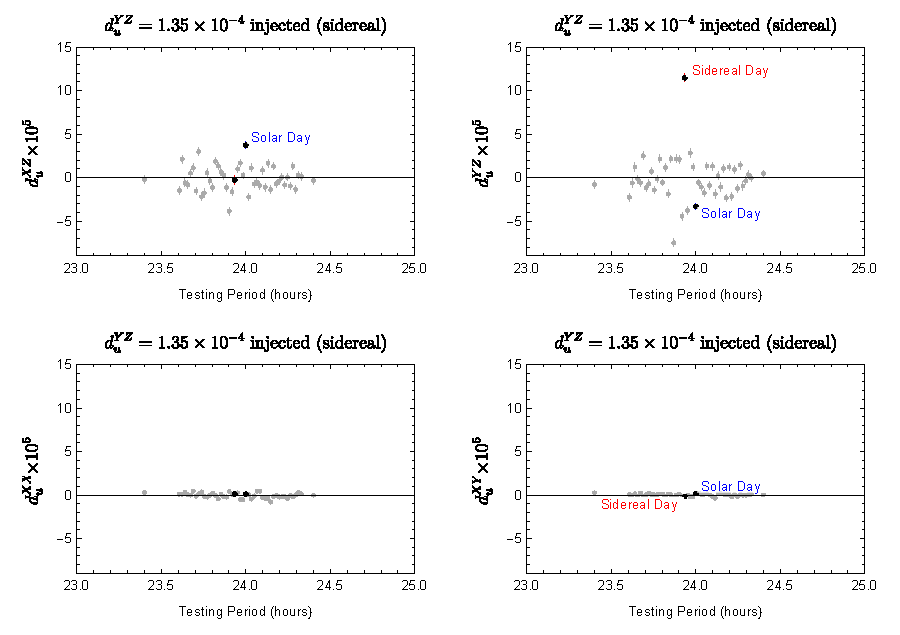
\includegraphics[width=0.8\textwidth]{figs/Mathematica-oldchi2/fit_duYZinjected_scan-narrow}
\caption{Sidereal signal injection ($d_u^{YZ} = 1.35 \times 10^{-4}$). Fit for the $d_u^{YZ}$ coefficient as a function of the testing phase. Red and blue fits correspond to the sidereal and solar testing phases.}
\label{fig:RD_sidereal_signal_scan}
\end{figure}



\subsection{Solar phase signal injection: recovery test}
\label{ssec:SolarInjectionRecovery}
%
Same as section~\ref{ssec:SiderealInjectionRecovery} but with a solar signal injected. Results are presented in figures~\ref{fig:RD_solar_signal}, \ref{fig:RD_solar_signal_fits_sidsol} and \ref{fig:RD_solar_signal_fits_1h}. \textcolor{red}{There is one feature of these results which I do not understand. Using a solar testing phase I find $\left[ d_u^{YZ}\right]_\text{fit} = (6.4 \pm 0.3) \times 10^{-5}$ which is a factor two smaller than the injected one.}

\begin{figure}[H]
\centering
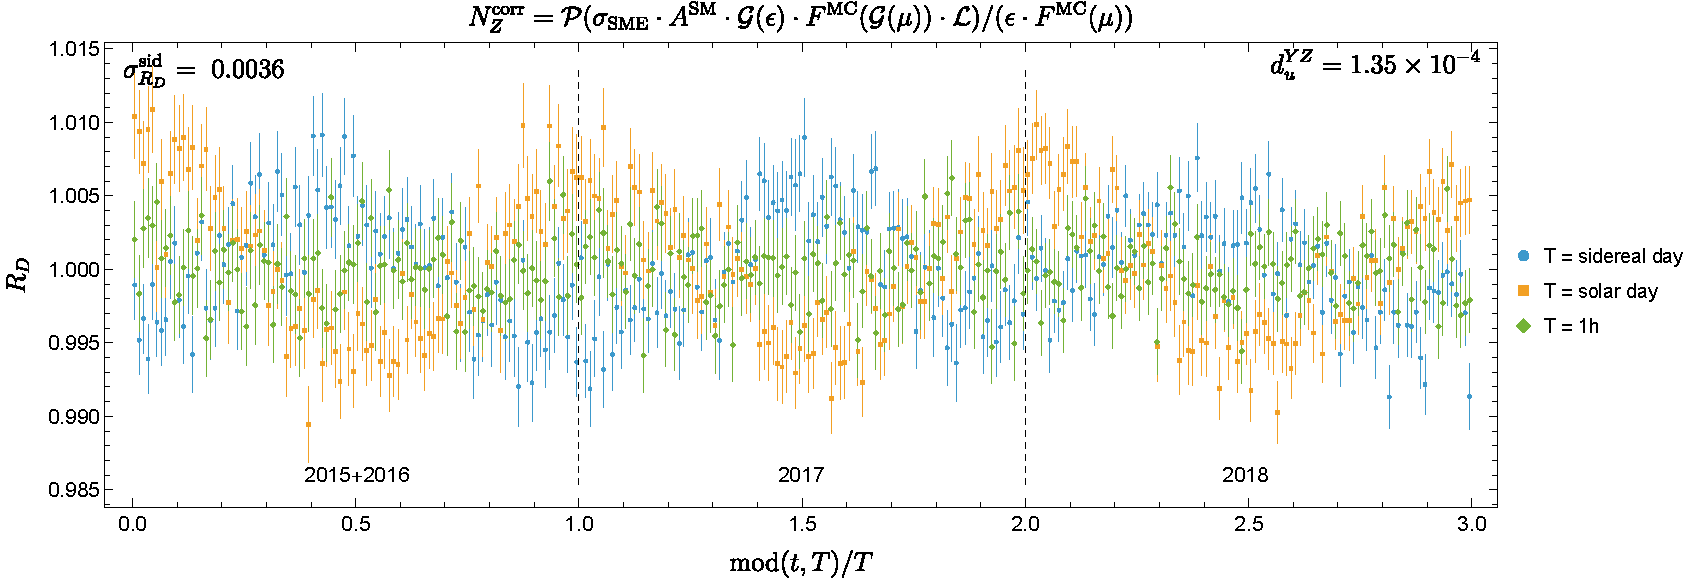
\includegraphics[width=\textwidth]{figs/Mathematica-oldchi2/xs(sigmaFIDSMEsolar eps FMC)_phase}
\caption{$R_D$ distribution with a solar signal injection ($d_u^{YZ} = 1.35 \times 10^{-4}$). In the upper right corner we show the standard deviation of the sidereal day distribution.}
\label{fig:RD_solar_signal}
\end{figure}

\begin{figure}[H]
\centering
\begin{minipage}[H]{\textwidth}
    \vspace{0pt}
    \centering
   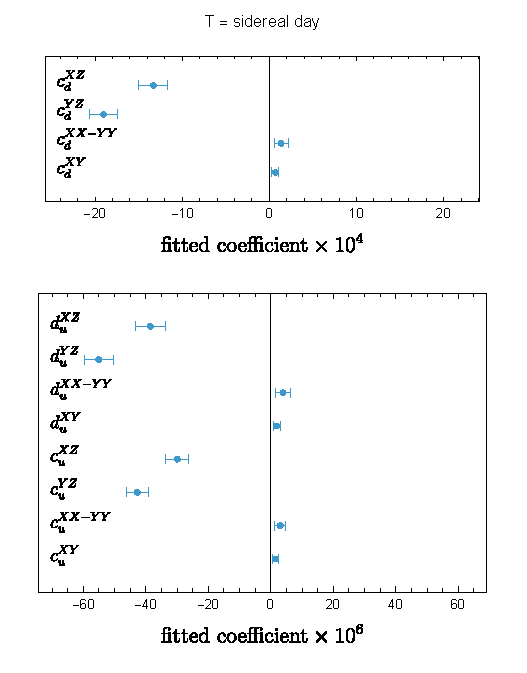
\includegraphics[width=0.49\textwidth]{figs/Mathematica-oldchi2/xs(sigmaFIDSMEsolar eps FMC)_fit_sday}
   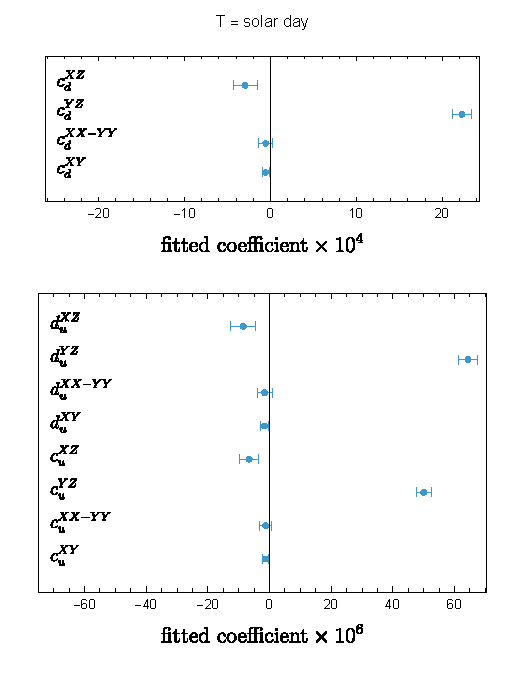
\includegraphics[width=0.49\textwidth]{figs/Mathematica-oldchi2/xs(sigmaFIDSMEsolar eps FMC)_fit_day}
\end{minipage}
\begin{minipage}[H]{\textwidth}
    \vspace{1.6cm}
    \centering
    \begin{tabular}{|l|c|}
        \hline
$d_u^{XZ}$ & $(-3.85 \pm 0.48)\times 10^{-5}$ \\
$d_u^{YZ}$ & $(-5.50 \pm 0.46)\times 10^{-5}$ \\
$d_u^{XX-YY}$ & $(3.9 \pm 2.3)\times 10^{-6}$ \\
$d_u^{XY}$ & $(1.9 \pm 1.1)\times 10^{-6}$ \\
$c_u^{XZ}$ & $(-2.99 \pm 0.37)\times 10^{-5}$ \\
$c_u^{YZ}$ & $(-4.27 \pm 0.36)\times 10^{-5}$ \\
$c_u^{XX-YY}$ & $(3.0 \pm 1.8)\times 10^{-6}$ \\
$c_u^{XY}$ & $(1.51 \pm 0.89)\times 10^{-6}$ \\
$c_d^{XZ}$ & $(-1.33 \pm 0.17)\times 10^{-3}$ \\
$c_d^{YZ}$ & $(-1.90 \pm 0.16)\times 10^{-3}$ \\
$c_d^{XX-YY}$ & $(1.35 \pm 0.81)\times 10^{-4}$ \\
$c_d^{XY}$ & $(6.7 \pm 4.0)\times 10^{-5}$ \\
                        \hline
        \end{tabular}
        \;\;\;\;\;\;\;\;\;\;\;\;\;\;\;\;\;\;
    \begin{tabular}{|l|c|}
        \hline
$d_u^{XZ}$ & $(-8.5 \pm 4.1)\times 10^{-6}$ \\
$d_u^{YZ}$ & $(6.44 \pm 0.32)\times 10^{-5}$ \\
$d_u^{XX-YY}$ & $(-1.6 \pm 2.4)\times 10^{-6}$ \\
$d_u^{XY}$ & $(-1.6 \pm 1.2)\times 10^{-6}$ \\
$c_u^{XZ}$ & $(-6.6 \pm 3.2)\times 10^{-6}$ \\
$c_u^{YZ}$ & $(5.00 \pm 0.25)\times 10^{-5}$ \\
$c_u^{XX-YY}$ & $(-1.2 \pm 1.9)\times 10^{-6}$ \\
$c_u^{XY}$ & $(-1.25 \pm 0.90)\times 10^{-6}$ \\
$c_d^{XZ}$ & $(-2.9 \pm 1.4)\times 10^{-4}$ \\
$c_d^{YZ}$ & $(2.23 \pm 0.11)\times 10^{-3}$ \\
$c_d^{XX-YY}$ & $(-5.5 \pm 8.4)\times 10^{-5}$ \\
$c_d^{XY}$ & $(-5.6 \pm 4.0)\times 10^{-5}$ \\
                                \hline
        \end{tabular}
\end{minipage}
\caption{Solar signal injection test ($d_u^{YZ} = 1.35 \times 10^{-4}$): fit results for sidereal (left) and solar (right) testing phases.}
\label{fig:RD_solar_signal_fits_sidsol}
\end{figure}


\begin{figure}[H]
\centering
\begin{minipage}[H]{0.49\textwidth}
    \vspace{1.6cm}
    \centering
    \begin{tabular}{|l|c|}
        \hline
$d_u^{XZ}$ & $(5.1 \pm 4.8)\times 10^{-6}$ \\
$d_u^{YZ}$ & $(6.8 \pm 4.8)\times 10^{-6}$ \\
$d_u^{XX-YY}$ & $(1.2 \pm 2.5)\times 10^{-6}$ \\
$d_u^{XY}$ & $(11. \pm 12.)\times 10^{-7}$ \\
$c_u^{XZ}$ & $(4.0 \pm 3.7)\times 10^{-6}$ \\
$c_u^{YZ}$ & $(5.3 \pm 3.7)\times 10^{-6}$ \\
$c_u^{XX-YY}$ & $(0.9 \pm 1.9)\times 10^{-6}$ \\
$c_u^{XY}$ & $(8.8 \pm 9.5)\times 10^{-7}$ \\
$c_d^{XZ}$ & $(1.8 \pm 1.7)\times 10^{-4}$ \\
$c_d^{YZ}$ & $(2.4 \pm 1.7)\times 10^{-4}$ \\
$c_d^{XX-YY}$ & $(4.1 \pm 8.5)\times 10^{-5}$ \\
$c_d^{XY}$ & $(3.9 \pm 4.2)\times 10^{-5}$ \\
        \hline
        \end{tabular}
\end{minipage}
\begin{minipage}[H]{0.49\textwidth}
    \vspace{0pt}
    \centering
   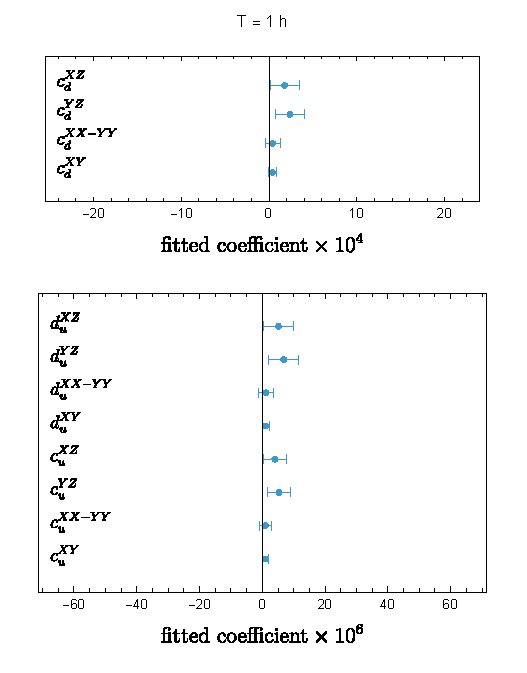
\includegraphics[width=\textwidth]{figs/Mathematica-oldchi2/xs(sigmaFIDSMEsolar eps FMC)_fit_1h}
\end{minipage}
\caption{Solar signal injection test ($d_u^{YZ} = 1.35 \times 10^{-4}$): fit results for 1 hr testing phase.}
\label{fig:RD_solar_signal_fits_1h}
\end{figure}


\subsection{Solar phase signal injection: scrambling}
\label{ssec:SolarInjectionScrambling}
%
In figures~\ref{fig:RD_solar_signal_scrambled} and \ref{fig:RD_solar_signal_scrambled_fits_sidsol}, we demonstrate that a random scrambling of all time stamps is sufficient to completely erase the presence of a strong solar signal.


\begin{figure}[H]
\centering
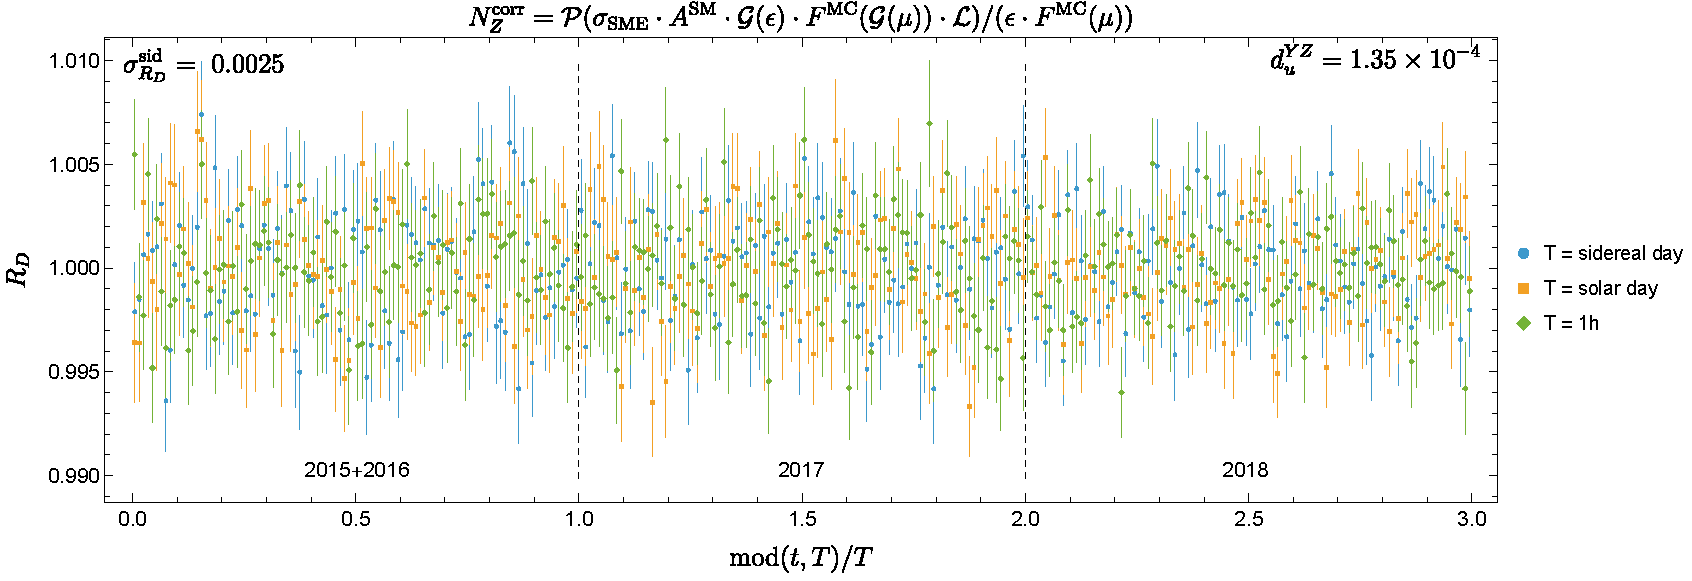
\includegraphics[width=\textwidth]{figs/Mathematica-oldchi2/xs(sigmaFIDSMEsolar eps FMC)_randomized_phase}
\caption{$R_D$ distribution with a solar signal injection ($d_u^{YZ} = 1.35 \times 10^{-4}$) after one scrambling. In the upper right corner we show the standard deviation of the sidereal day distribution.}
\label{fig:RD_solar_signal_scrambled}
\end{figure}


\begin{figure}[H]
\centering
\begin{minipage}[H]{\textwidth}
    \vspace{0pt}
    \centering
   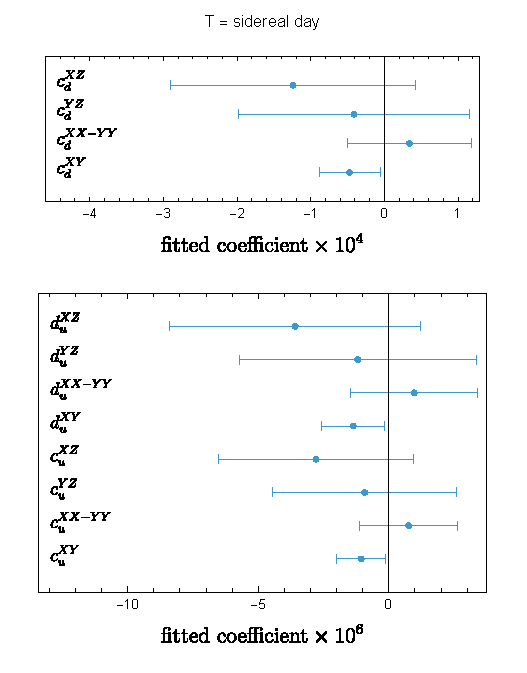
\includegraphics[width=0.49\textwidth]{figs/Mathematica-oldchi2/xs(sigmaFIDSMEsolar eps FMC)_randomized_fit_sday}
   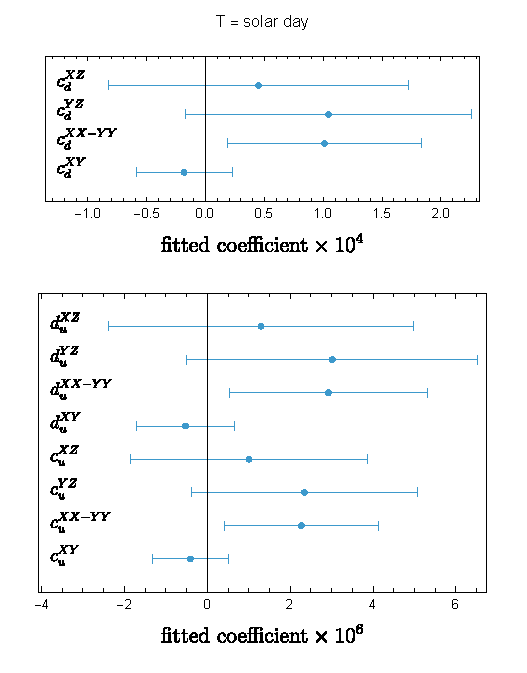
\includegraphics[width=0.49\textwidth]{figs/Mathematica-oldchi2/xs(sigmaFIDSMEsolar eps FMC)_randomized_fit_day}
\end{minipage}
\begin{minipage}[H]{\textwidth}
    \vspace{1.6cm}
    \centering
    \begin{tabular}{|l|c|}
        \hline
$d_u^{XZ}$ & $(-3.6 \pm 4.8)\times 10^{-6}$ \\
$d_u^{YZ}$ & $(-1.2 \pm 4.5)\times 10^{-6}$ \\
$d_u^{XX-YY}$ & $(1. \pm 2.4)\times 10^{-6}$ \\
$d_u^{XY}$ & $(-14. \pm 12.)\times 10^{-7}$ \\
$c_u^{XZ}$ & $(-2.8 \pm 3.7)\times 10^{-6}$ \\
$c_u^{YZ}$ & $(-0.9 \pm 3.5)\times 10^{-6}$ \\
$c_u^{XX-YY}$ & $(0.8 \pm 1.9)\times 10^{-6}$ \\
$c_u^{XY}$ & $(-10.6 \pm 9.3)\times 10^{-7}$ \\
$c_d^{XZ}$ & $(-1.2 \pm 1.7)\times 10^{-4}$ \\
$c_d^{YZ}$ & $(-0.4 \pm 1.6)\times 10^{-4}$ \\
$c_d^{XX-YY}$ & $(3.4 \pm 8.4)\times 10^{-5}$ \\
$c_d^{XY}$ & $(-4.7 \pm 4.1)\times 10^{-5}$ \\
                \hline
        \end{tabular}
        \;\;\;\;\;\;\;\;\;\;\;\;\;\;\;\;\;\;
    \begin{tabular}{|l|c|}
        \hline
$d_u^{XZ}$ & $(1.3 \pm 3.7)\times 10^{-6}$ \\
$d_u^{YZ}$ & $(3.0 \pm 3.5)\times 10^{-6}$ \\
$d_u^{XX-YY}$ & $(2.9 \pm 2.4)\times 10^{-6}$ \\
$d_u^{XY}$ & $(-5. \pm 12.)\times 10^{-7}$ \\
$c_u^{XZ}$ & $(1.0 \pm 2.9)\times 10^{-6}$ \\
$c_u^{YZ}$ & $(2.3 \pm 2.7)\times 10^{-6}$ \\
$c_u^{XX-YY}$ & $(2.3 \pm 1.9)\times 10^{-6}$ \\
$c_u^{XY}$ & $(-4.1 \pm 9.2)\times 10^{-7}$ \\
$c_d^{XZ}$ & $(0.4 \pm 1.3)\times 10^{-4}$ \\
$c_d^{YZ}$ & $(1.0 \pm 1.2)\times 10^{-4}$ \\
$c_d^{XX-YY}$ & $(10.1 \pm 8.3)\times 10^{-5}$ \\
$c_d^{XY}$ & $(-1.8 \pm 4.1)\times 10^{-5}$ \\
                        \hline
        \end{tabular}
\end{minipage}
\caption{Solar signal injection test ($d_u^{YZ} = 1.35 \times 10^{-4}$) after one scrambling of all time stamps: fit results for sidereal (left) and solar (right) testing phases.}
\label{fig:RD_solar_signal_scrambled_fits_sidsol}
\end{figure}

\subsection{Solar phase signal injection: scan over the testing phase}
\label{ssec:SolarInjectionScan}
%
In this section we study, as a function of the testing phase, the extraction of the coefficient $d_u^{YZ}$ from a sample in which a $d_u^{YZ} = 1.35 \times 10^{-4}$ solar signal has been injected. The results of this test is presented in figure~\ref{fig:RD_solar_signal_scan} (the four lower panels focus on the restricted [23 hr, 25 hr] range). Around the sidereal and solar phases we scan the testing phase with a granularity of 1 min (going below this is problematic because the average LB duration is about 1 min). 

\begin{figure}[H]
\centering
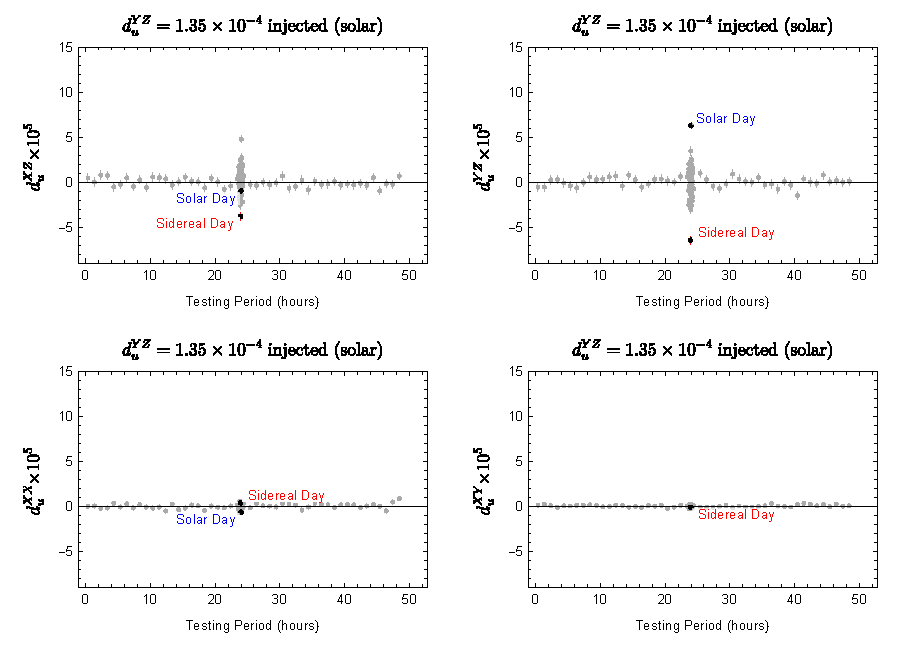
\includegraphics[width=0.8\textwidth]{figs/Mathematica-oldchi2/fit_duYZinjected_solar_scan-wide}
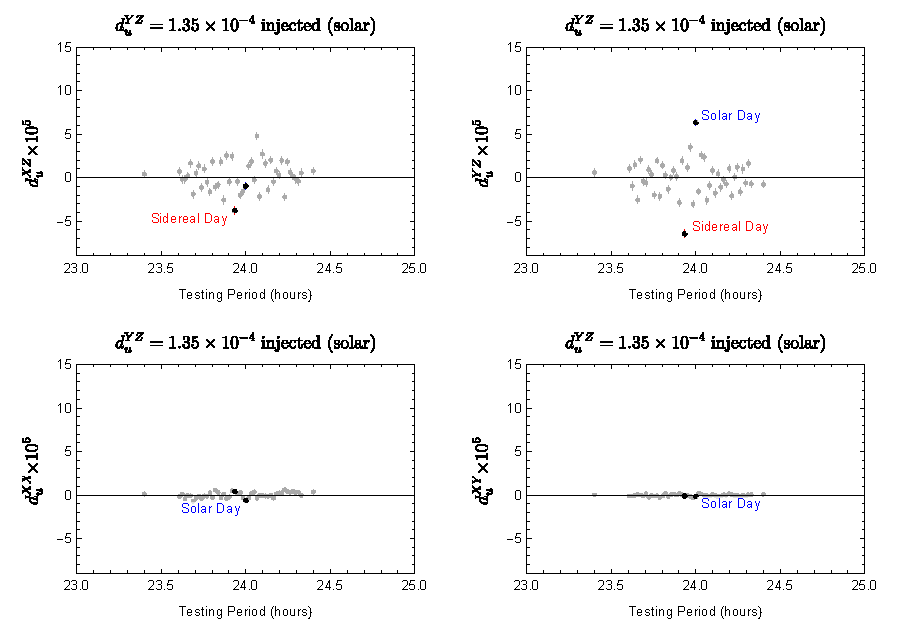
\includegraphics[width=0.8\textwidth]{figs/Mathematica-oldchi2/fit_duYZinjected_solar_scan-narrow}
\caption{Solar signal injection ($d_u^{YZ} = 1.35 \times 10^{-4}$). Fit for the $d_u^{YZ}$ coefficient as a function of the testing phase. Red and blue fits correspond to the sidereal and solar testing phases.}
\label{fig:RD_solar_signal_scan}
\end{figure}

